%Este trabalho está licenciado sob a Licença Atribuição-CompartilhaIgual 4.0 Internacional Creative Commons. Para visualizar uma cópia desta licença, visite http://creativecommons.org/licenses/by-sa/4.0/deed.pt_BR ou mande uma carta para Creative Commons, PO Box 1866, Mountain View, CA 94042, USA.

\chapter{Cônicas}\label{cap_conicas}
\thispagestyle{fancy}

\section{Elipse}\label{cap_conicas_sec_elipse}

Sejam $F_1,F_2$ pontos sobre um plano $\pi$, $c$ a distância entre $c_1$ e $c_2$ e $a > c$. Chama-se \emph{elipse} de \emph{focos} $F_1$ e $F_2$ ao conjunto de pontos $P$ tais que
\begin{equation}
  |PF_1| + |PF_2| = 2a.
\end{equation}
Veja a Figura \ref{fig:elipse}.

\begin{figure}[H]
  \centering
  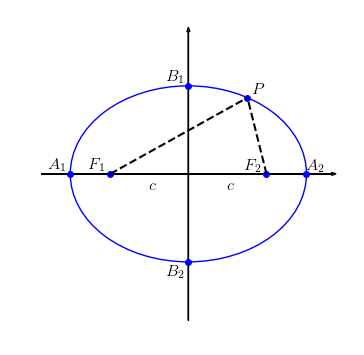
\includegraphics[width=0.7\textwidth]{./cap_conicas/dados/fig_elipse/fig_elipse}
  \caption{Ilustração de uma elipse de focos $F_1$ e $F_2$.}
  \label{fig:elipse}
\end{figure}

Dada uma tal elipse, identificamos $2c=|F_1F_2|$ como a \emph{distância focal}. Os pontos $A_1$ e $A_2$ de interseção da elipse com a reta que passa pelos focos são chamados de \emph{vértices} da elipse. O segmento $A_1A_2$ é chamado de \emph{eixo maior} da elipse. Observamos que
\begin{equation}
  |A_1A_2| = 2a.
\end{equation}
O ponto médio do segmento $F_1F_2$ é chamado de \emph{centro} da elipse. Sejam $B_1$ e $B_2$ os pontos de interseção da elipse com a reta que passa pelo centro da elipse e é perpendicular ao segmento $A_1A_2$. Assim sendo, o segmento $B_1B_2$ é chamado de \emph{eixo menor} da elipse. Vamos denotar
\begin{equation}
  2b = |B_1B_2|.
\end{equation}

Chamamos de \emph{excentricidade} da elipse o número
\begin{equation}
  e = \frac{c}{a}.
\end{equation}
Notemos que $0 \leq e < 1$. Para $e=0$, temos $c=0$ e, portanto $F_1=F_2$. Neste caso, a elipse é a circunferência de centro em $F_1$ (ou $F_2$) e diâmetro $2a$. No que $e$ tende a $1$, a elipse tende ao segmento $A_1A_2$.

Por fim, notemos que o triângulo $B_1OF_2$ é retângulo, $|OF_2|=c$, $|F_2B_1|=a$ e $|OB_1|=b$. Do teorema de Pitágoras segue
\begin{equation}\label{eq:elipse_obs}
  b^2 + c^2 = a^2.
\end{equation}

\subsection{Equação reduzida da elipse}

Consideremos o sistema de coordenadas cartesianas. Sejam $F_1=(-c,0)$ e $F_2=(c,0)$, $c\geq 0$, os focos de uma dada elipse (veja a Figura \ref{fig:elipse}).  Se $P=(x,y)$ é um ponto da elipse, então
\begin{equation}
  |PF_1| + |PF_2| = 2a.
\end{equation}
Como
\begin{align}
  |PF_1| &= \sqrt{(x+c)^2 + y^2}, \\
  |PF_2| &= \sqrt{(x-c)^2 + y^2},
\end{align}
temos
\begin{equation}
  \sqrt{(x+c)^2 + y^2} + \sqrt{(x-c)^2 + y^2} = 2a,
\end{equation}
ou, equivalentemente,
\begin{equation}
  \sqrt{(x+c)^2 + y^2} = 2a - \sqrt{(x-c)^2 + y^2}.
\end{equation}
Elevando ao quadrado, obtemos
\begin{equation}
  (x+c)^2 + y^2 = 4a^2 - 4a\sqrt{(x-c)^2+y^2} + (x-c)^2+y^2.
\end{equation}
Por cancelamento e rearranjo dos termos, obtemos
\begin{equation}
  a\sqrt{(x-c)^2+y^2}=a^2-cx.
\end{equation}
Elevando novamente ao quadrado, temos
\begin{equation}
  a^2(x-c)^2+a^2y^2=a^4-2a^2cx+c^2x^2,
\end{equation}
donde
\begin{equation}
  a^2x^2 -2a^2cx + a^2c^2 + a^2y^2= a^4 -2a^2cx + c^2x^2.
\end{equation}
Por cancelamento e rearranjo dos termos, obtemos
\begin{equation}
  x^2(a^2 - c^2) + a^2y^2 = a^2(a^2 - c^2).
\end{equation}
Como $a>c$, dividimos por $a^2-c^2$  e depois por $a^2$ para obtemos
\begin{equation}
  \frac{x^2}{a^2} + \frac{y^2}{a^2-c^2} = 1.
\end{equation}
Por fim, da equação \eqref{eq:elipse_obs}, temos $a^2-c^2 = b^2$, o que nos leva  a \emph{equação reduzida da elipse}
\begin{equation}
  \frac{x^2}{a^2} - \frac{y^2}{b^2} = 1.
\end{equation}

\emconstrucao

\section{Hipérbole}\label{cap_conicas_sec_hiperbole}

\emconstrucao

\section{Parábola}\label{cap_conicas_sec_parabola}

\emconstrucao